En esta sección se describen las interacciones multijugador implementadas en el juego, 
que permiten a los jugadores interactuar entre sí de diversas formas, fomentando la cooperación, 
la competencia y la socialización dentro del mundo del juego.

\subsubsection{Chat en el juego}
Se ha implementado un sistema de chat en el juego que permite a los jugadores comunicarse entre sí en tiempo real. 
El chat es un único canal de comunicación donde los players pueden ver sus mensajes y los de otros jugadores, 
mostrandose visualmente sobre cada personaje. El sistema de chat es sencillo pero efectivo, permitiendo 
a los jugadores coordinarse, compartir información y socializar mientras juegan.

\begin{figure}[H]
    \centering
    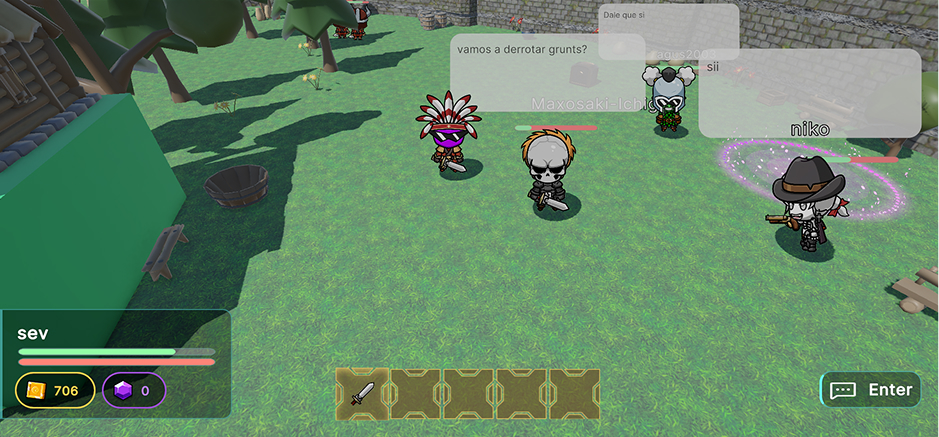
\includegraphics[width=0.85\textwidth]{img/08-implemented-solution/product/chat.jpg}
    \caption{Captura de pantalla del sistema de chat en el juego}
    \label{fig:chat}
\end{figure}

\subsubsection{Combate}
El juego incluye un sistema de combate que permite a los jugadores enfrentarse entre sí en duelos o en batallas grupales. 
Los jugadores pueden adoptar distintas estrategias de combate según el sistema de armas disponibles. 
Si bien el sistema de combate está diseñado para ser justo y equilibrado, depende de como se ha diseñado el mundo 
donde se encuentran los jugadores, ya que los items, sean armas o consumibles, tienen sus propias estadísticas 
y características cambiando el comportamiento de cada jugador en combate.

Los tipos de combate disponibles incluyen ataques cuerpo a cuerpo desarmado, con armas de cuerpo a cuerpo y 
con armas de ataques a distancia. El sistema de combate cercano utiliza un sistema de colisiones para determinar 
si un ataque ha impactado a un oponente alrededor del area hacia donde mira el personaje, mientras que el 
combate a distancia se basa en detección de objetivos a traves de una trayectoria trazada visualmente que impacta 
instantáneamente al objetivo.

Por el momento el combate entre jugadores siempre está activo, lo que significa que los jugadores pueden atacarse 
entre sí en cualquier momento. Los NPCs pasivos no pueden atacar ni ser atacados, pero los NPCs agresivos 
(o \textit{Enemies}) pueden atacar a los jugadores y ser atacados por ellos. Los enemigos atacarán a los 
jugadores que entren en su área de detección, y su ataque está también ligado al arma que el creador del 
mundo le haya asignado.


\begin{figure}[H]
    \centering
    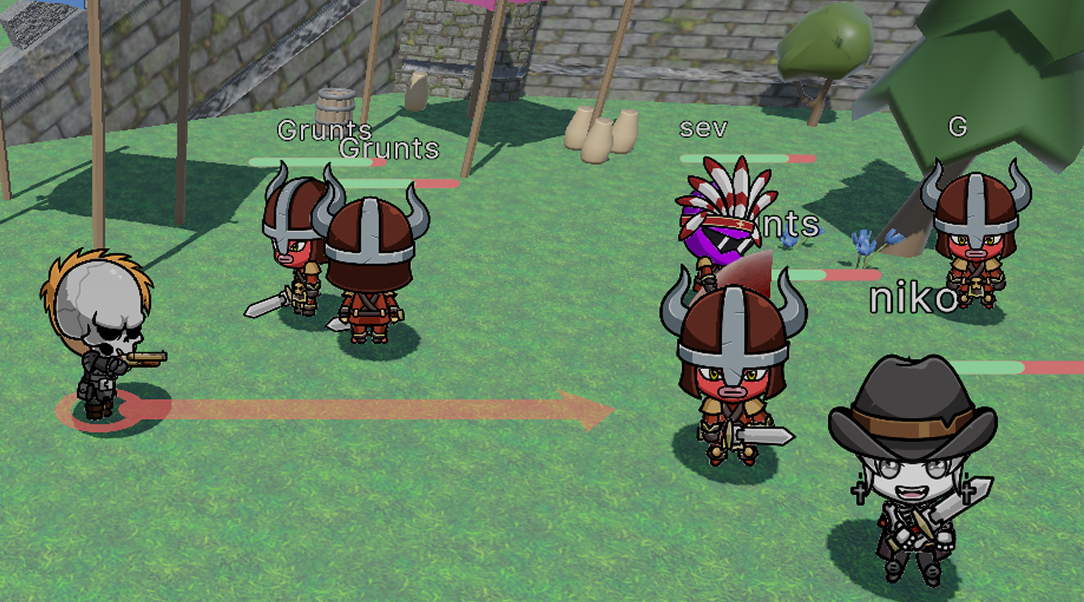
\includegraphics[width=0.85\textwidth]{img/08-implemented-solution/product/combat.jpg}
    \caption{Captura de pantalla del sistema de combate en el juego}
    \label{fig:combat}
\end{figure}


